% =============================================================================
%  Breadcrumbs — Figure 4
%  Federated continual learning on the synthetic document corpus.
%
%  This figure answers the weakness the report states in Section 7.3: that the
%  simulation in Figure 3 runs on Gaussian clusters whose classes differ mainly
%  in their mean, so a compact summary of those means carries most of the signal
%  and prototype replay could look good for a reason that has nothing to do with
%  the method.
%
%  These numbers are measured on the row-level corpus instead: 19,980 documents
%  across five record types, nine anomaly kinds and six sites, with the six
%  sites as federated clients (Dirichlet alpha = 0.6) and the three violation
%  waves as continual stages. Balanced accuracy, five seeds, measured at a
%  chosen 10% false-positive budget rather than at whatever point argmax lands
%  on -- see tab4_corpus.tex for the full operating-point curve.
%
%  Regenerate with:  python -m model.run train --rounds 15 --seeds 5
%  Source of truth:  Breadcrumbs Project/model/artefacts/training.json
%
%  HOW TO COMPILE
%    Standalone, pdfLaTeX. Drawn entirely in TikZ; no image files needed.
% =============================================================================
%  NOTE ON DUPLICATION
%    main.tex carries an inlined copy of this content, because the paper draws
%    every figure in TikZ so that nothing has to be uploaded alongside it. This
%    standalone file exists for previewing one figure without compiling the whole
%    report. If you change the numbers, change both, or the preview will disagree
%    with the paper. Regenerate from model/artefacts/training.json.
\documentclass[11pt,border=6pt,varwidth=20cm]{standalone}

\usepackage[T1]{fontenc}
\usepackage[utf8]{inputenc}
\usepackage{lmodern}
\usepackage{amsmath,amssymb}
\usepackage{xcolor}
\usepackage{tikz}
\usepackage{pgfplots}
\pgfplotsset{compat=1.18}

% ---- palette (colour-blind safe, prints correctly in greyscale) -------------
\definecolor{tcblue}{HTML}{2563EB}
\definecolor{tcorange}{HTML}{E8710A}
\definecolor{tcgreen}{HTML}{059669}
\definecolor{tcgrey}{HTML}{6B7280}
\definecolor{tctext}{HTML}{111827}
\definecolor{tcline}{HTML}{E5E7EB}

\begin{document}
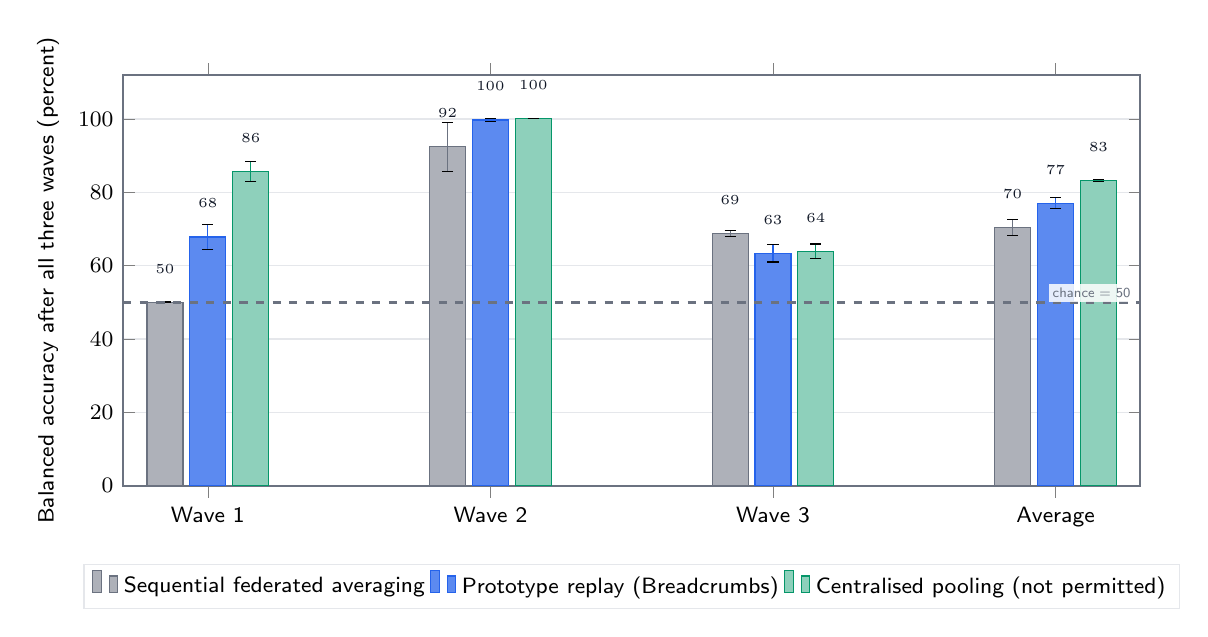
\begin{tikzpicture}
\begin{axis}[
  width=14.5cm, height=6.8cm,
  ybar=2.5pt, bar width=13pt,
  font=\sffamily\small,
  ymin=0, ymax=112, ytick={0,20,40,60,80,100},
  ylabel={Balanced accuracy after all three waves (percent)},
  symbolic x coords={Wave 1, Wave 2, Wave 3, Average},
  xtick=data,
  ymajorgrids=true, grid style={tcline,line width=0.5pt},
  axis line style={tcgrey,line width=0.6pt},
  tick label style={font=\sffamily\footnotesize},
  label style={font=\sffamily\footnotesize},
  legend style={font=\sffamily\footnotesize,at={(0.5,-0.19)},anchor=north,
                legend columns=3,draw=tcline},
  nodes near coords, every node near coord/.append style={
      font=\sffamily\tiny,color=tctext,yshift=7pt,
      /pgf/number format/fixed,/pgf/number format/precision=0},
  error bars/y dir=both, error bars/y explicit,
]
% Sequential federated averaging: wave 1 collapses to chance on every seed.
\addplot[fill=tcgrey!55,draw=tcgrey] coordinates {
  (Wave 1,50.0) +- (0,0.1) (Wave 2,92.4) +- (0,6.7)
  (Wave 3,68.8) +- (0,0.9) (Average,70.4) +- (0,2.1)};
% Prototype replay, ledger-anchored memory bank.
\addplot[fill=tcblue!75,draw=tcblue] coordinates {
  (Wave 1,67.8) +- (0,3.4) (Wave 2,99.7) +- (0,0.5)
  (Wave 3,63.4) +- (0,2.4) (Average,77.0) +- (0,1.5)};
% Centralised pooling: the ceiling, and not permitted in the deployed system.
\addplot[fill=tcgreen!45,draw=tcgreen] coordinates {
  (Wave 1,85.7) +- (0,2.7) (Wave 2,100.0) +- (0,0.0)
  (Wave 3,63.9) +- (0,2.0) (Average,83.2) +- (0,0.3)};
\draw[tcgrey,dashed,line width=0.9pt]
  ({rel axis cs:0,0}|-{axis cs:Wave 1,50}) -- ({rel axis cs:1,0}|-{axis cs:Wave 1,50});
% Filled, so the note stays legible where it crosses a bar.
\node[font=\sffamily\tiny,text=tcgrey,anchor=south east,
      fill=white,fill opacity=0.85,text opacity=1,inner sep=1.5pt]
  at ({rel axis cs:0.995,0}|-{axis cs:Wave 1,50}) {chance = 50};
\legend{Sequential federated averaging, Prototype replay (Breadcrumbs),
        Centralised pooling (not permitted)}
\end{axis}
\end{tikzpicture}
\end{document}
